\chapter{Methodology}
In this chapter, the methodologies and tools for preparing the dataset, designing the model and experiment will be introduced. 
\section{Dataset Preparation}
    \subsection{Generate dataset manually}
    The stereo vision camera, fixed on the workbench, is implemented for takes pictures of wire harness \autoref{stereoCamera1}. Once the photograph is completed, the images will be uploaded and stored 
    in the bucket to the database MinIO.
    \begin{figure}
        \centering
        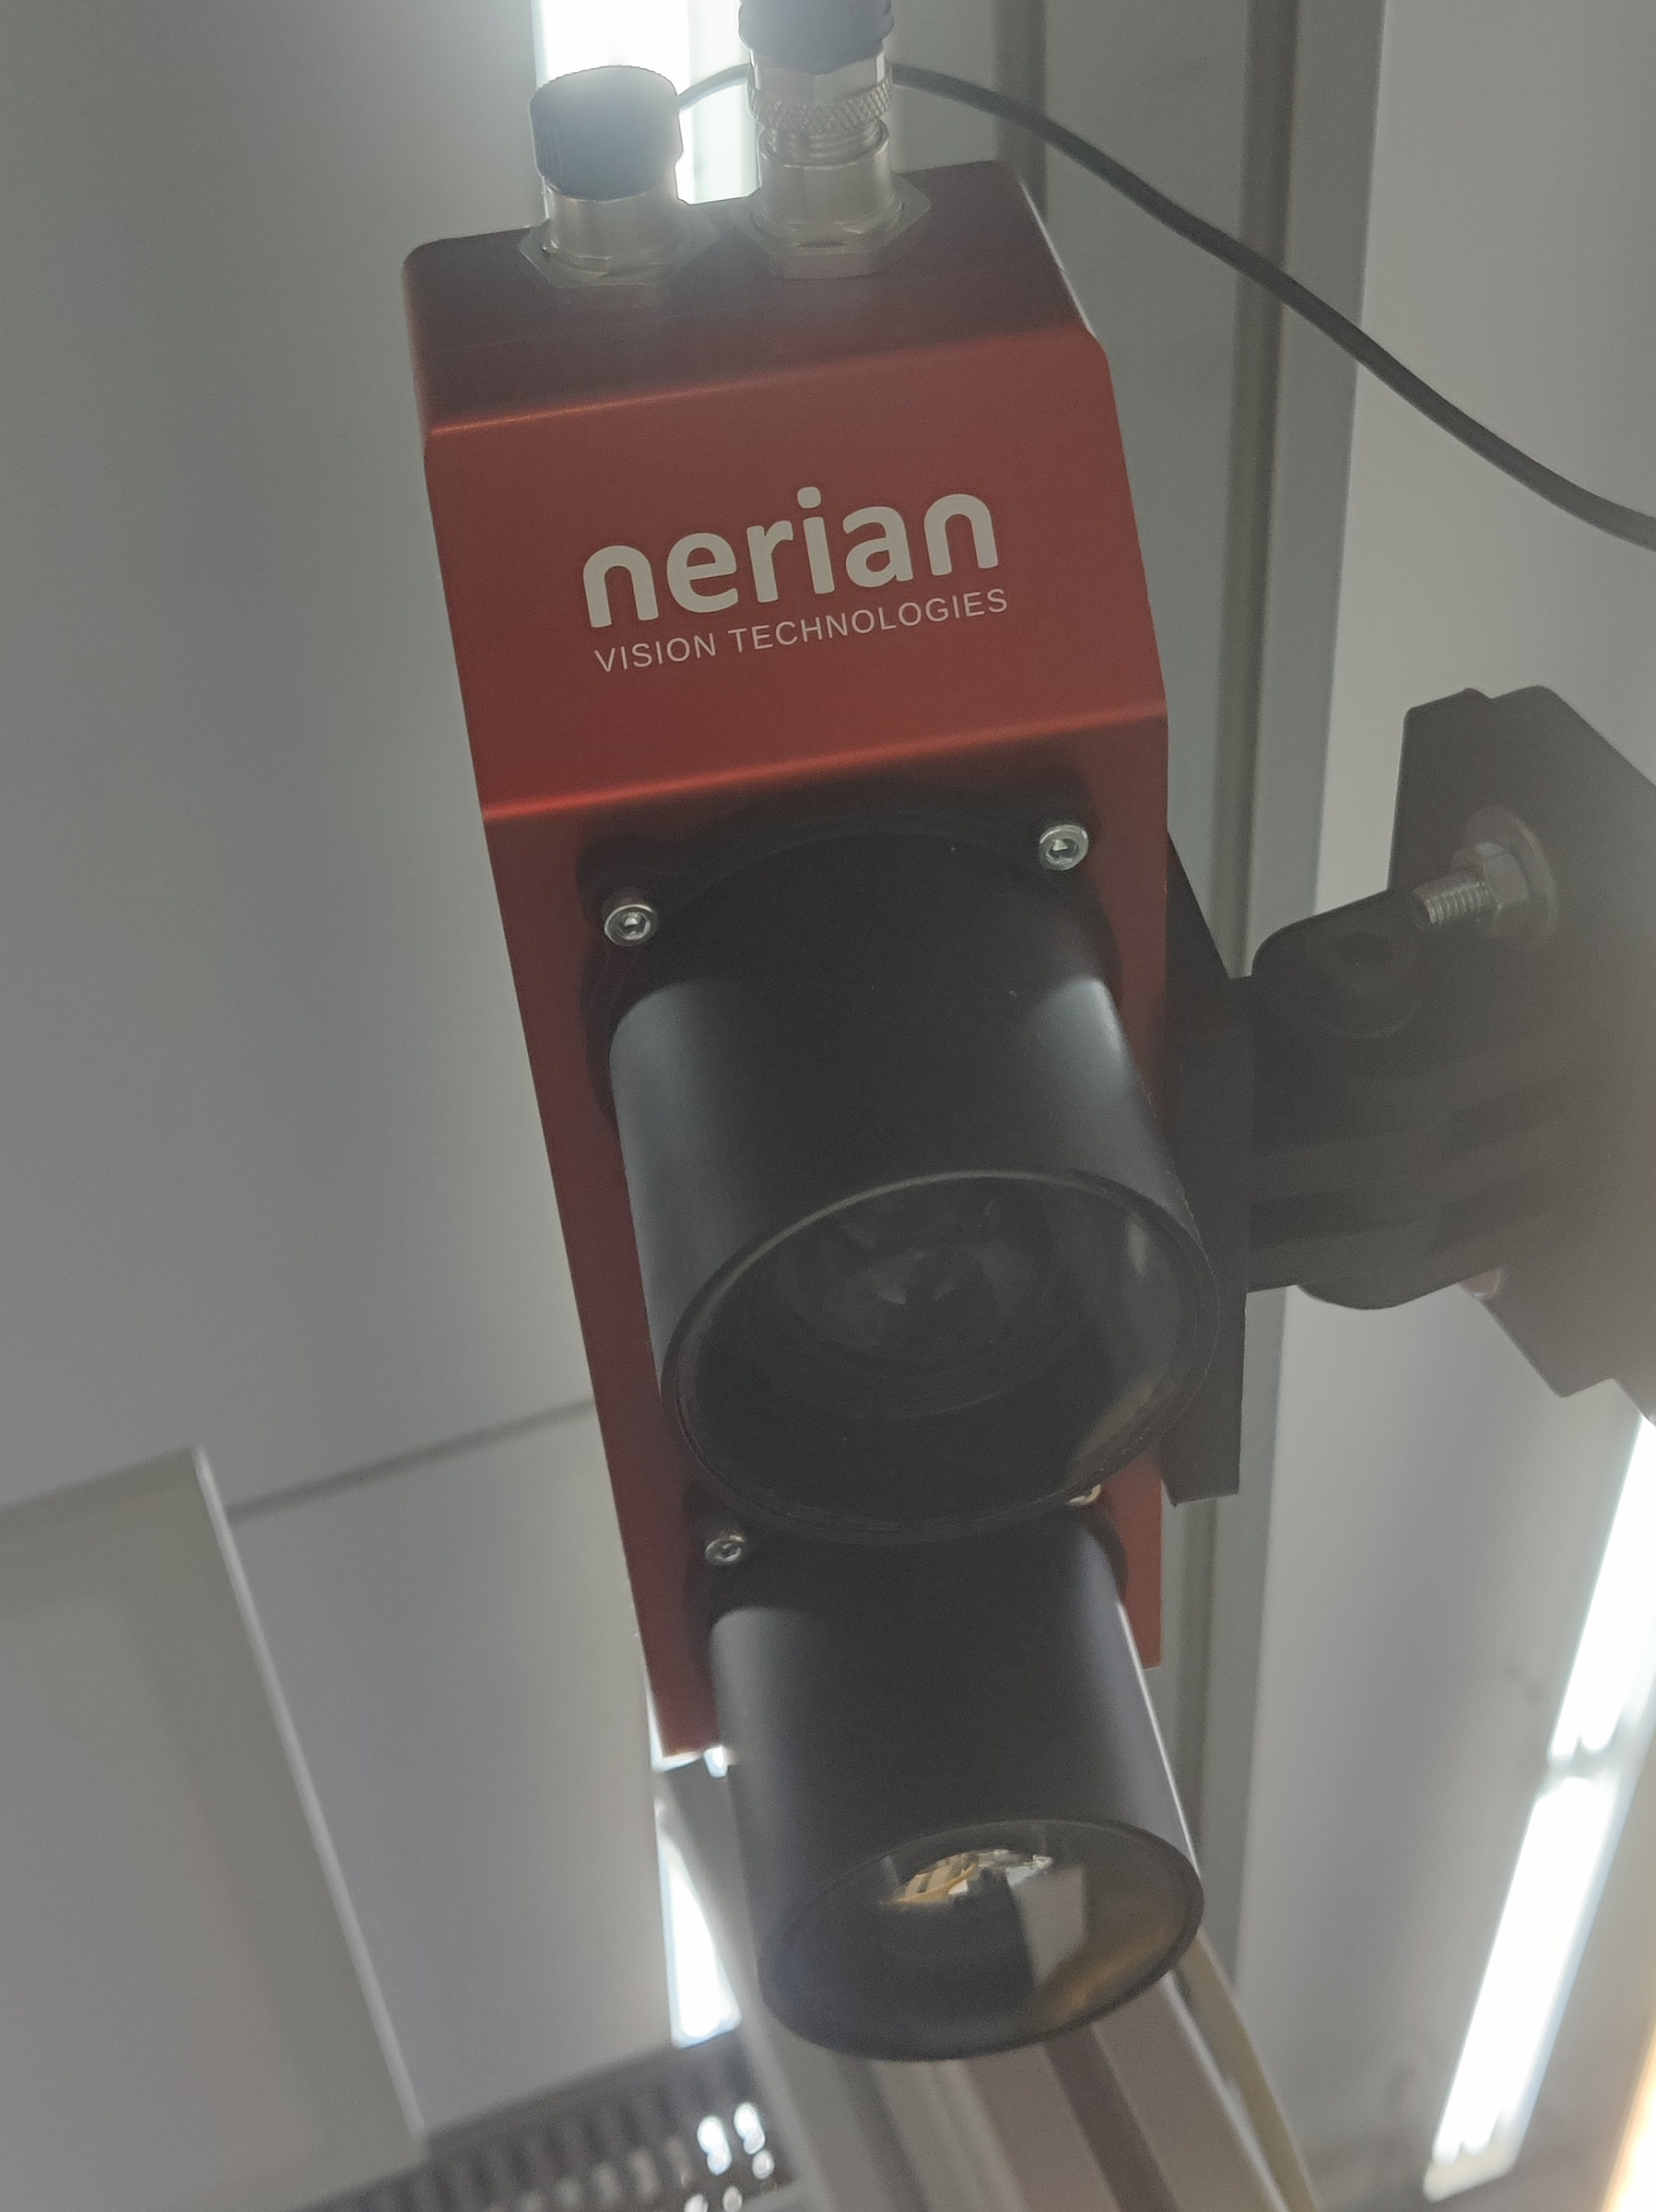
\includegraphics[width=0.4\linewidth]{example_images/stereoCamera1.jpg}
        \caption{Stereo Vision Camera}
        \label{stereoCamera1}
    \end{figure}
    Label studio\cite{LabelStudio} is a popular open-source data labeling tool. It could annotate for different vision tasks, e.g., keypoint detection, object segmentation, image classification.
    Howerver, the goal of this thesis is to construct the spline model of the wire harness by interpolating the keypoints, while the Label studio could only show the annotated keypoints in image.
    An annotation tool is developed through NiceGUI\cite{schindler2024nicegui}, which is a python-based UI framework and will show up in the web browser. The web interface of the annotation tool'
    is shown in \autoref{Annotation tool}. The user could select the bucket in dataset and load the images in this tool. Once the images are loaded, the annotation could begin.
    Click on the segment of the wire harness to create nodes. When there are more than four nodes on the segment, the cubic spline is 
    automatically interpolated. The positions of $n+1$ nodes are defined as $(x_k, y_k)$ for $k = 1, 2, ...n+1$, then the cubic spline between nodes $(x_k, y_k)$ and $(x_{k+1}, y_{k+1})$ is shown in
    \autoref{eq:cubic spline}. The neighboring splines need to fulfill the first and second order boundary conditions in \autoref{eq:boundary conditions}. 
    \begin{equation}
        \begin{aligned}
            &s_k(x) =  c_{k,3}x^3+c_{k,2}x^2+c_{k,1}x+c_{k,0}\\
            &s_k(x_k) = y_k,  s_k(x_{k+1}) = y_{k+1}
            \label{eq:cubic spline}
        \end{aligned}
    \end{equation}
    \begin{equation}
        \begin{aligned}
            s_k'(x_{k+1}) &= s_{k+1}'(x_{k+1})\\
            s_k''(x_{k+1}) &= s_{k+1}''(x_{k+1})
            \label{eq:boundary conditions}
        \end{aligned}
    \end{equation}
    The length and bending energy of the spline are calculated. The spline curve actually consists of numerous points.  The length of the entire spline curve 
    is obtained by summing the Euclidean distances of neighboring discrete points. The algorithm is shown in \autoref{Calculate the length of a spline}.
    \begin{algorithm} 
        \caption{Calculate the length of a spline}
        \label{Calculate the length of a spline}
        \begin{algorithmic}[1]
        \STATE \textbf{Input:} $X$
        \STATE $Length \leftarrow [\quad]$
        \FOR{$(x_{k},y_{k}),(x_{k+1},y_{k+1}) \in X$}
            \STATE $Distance \leftarrow \sqrt{(x_{k+1}-x_{k})^2+(y_{k+1}-y_{k})^2}$
            \STATE $Length.append(Distance)$
        \ENDFOR
        \RETURN $\text{sum}(Length)$
        \end{algorithmic}
    \end{algorithm}
    The benging energy is calcultated as \autoref{eq:bending energy}, where $\kappa(s)$ is the curvature of the spline as a function of the arc length s.
    \begin{equation}
        \begin{aligned}
            E = \int_{0}^{L} \kappa(s)^2ds
            \label{eq:bending energy}
        \end{aligned}
    \end{equation}
    The spline is defined in parametric form as $s(t) = (x(t),y(t))$ and the curvature spline be calculated as \autoref{eq:curvature}. 
    \begin{equation}
        \begin{aligned}
            \kappa(t) = \frac{\dot{x}(t) \ddot{y}(t) - \dot{y}(t) \ddot{x}(t)}{(\dot{x}(t)^2 + \dot{y}(t)^2)^{3/2}}
            \label{eq:curvature}
        \end{aligned}
    \end{equation}
    The whole equation could be represented in discrete form in \autoref{eq:curvature discrete form}.
    \begin{equation}
        \begin{aligned}
            E = \int_{0}^{L} \kappa(s)^2 \, ds = \int_{t_0}^{t_1} \kappa(t)^2 \left( \sqrt{\dot{x}(t)^2 + \dot{y}(t)^2} \right) \, dt
            \label{eq:curvature discrete form}
        \end{aligned}
    \end{equation}
    After one branch is labeled, the user could press up key to start labeling the next segment. The number of nodes on each segment should be the same. The sequences of 
    segments could also be adjusted. This is important for the model to learn the structure of the wire harness when the segments are not sorted in the program or the complexity 
    is too high to sort. Once all the segments are labeled, the annotations could be saved and exported as json file.
    \begin{figure}{!htbp}
        \centering
        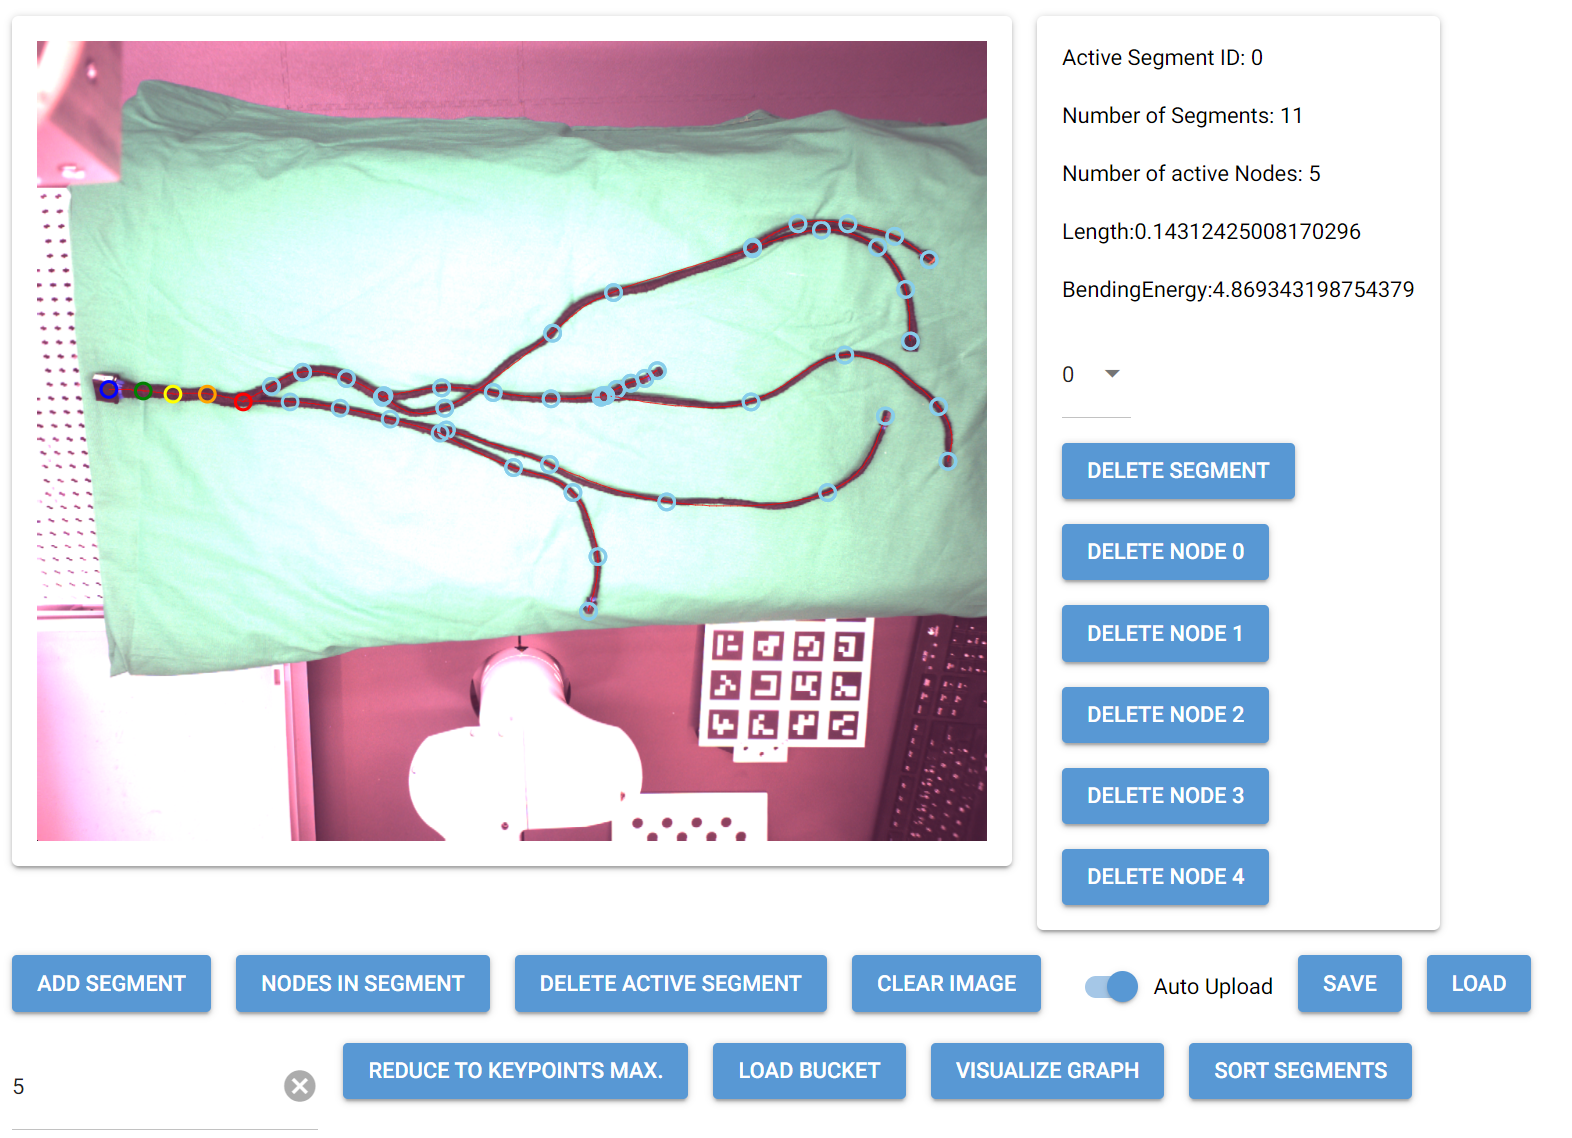
\includegraphics[width=0.9\linewidth]{example_images/NiceGUIInterface.png}
        \caption{Annotation tool}
        \label{Annotation tool}
    \end{figure}
\subsection{Dataset Expansion}
    Last subsection shows the approach of generating the dataset of the wire harness by using stereo vision camera and the annotation tool. However, annotating a large  
    dataset manually is time-consuming and inefficient. A small dataset could lead to the problem of under-fitting and the bad generalization. In this subsection, two 
    developed methods for expanding the datasets are introduced. 
\subsubsection{Synthetic images of BDLOs}
    A synthetic dataset of the eleven-segment wire harnesses is generated for transfer learning, which has the same topology as \autoref{fig:Topology of the eleven-segment wire harness}.
    To set up the configuration, the topology, the number of keypoints and the length of each segment are defined in advance. The cubic spline is obtained by interpolating randomly generated 
    control points under certain constraints, e.g. the maximum angle between two neighboring keypoints is set in \autoref{The constraint of maximum angle between two neighboring keypoints}
    to prevent the interpolating spline from being too curved. 
    \begin{figure}[!htbp]
        \centering
        \includegraphics[width=0.5\linewidth]{example_figures/MaxAngle_synthetic.pdf}
        \caption{The constraint of maximum angle between two neighboring keypoints}
        \label{The constraint of maximum angle between two neighboring keypoints}
    \end{figure}
    To make the fake image a better representation of some special situations such as overlapping, the lighting condition is mimic
    by means of a convolutional kernel to minimize the gap between the real and fake images. From the edges to the center of the segment, the pixel become lighter in color. An example of the 
    synthetic wire harness is shown in \autoref{An example of the synthetic image of the eleven-segment wire harness}.
    \begin{figure}[!htbp]
        \centering
        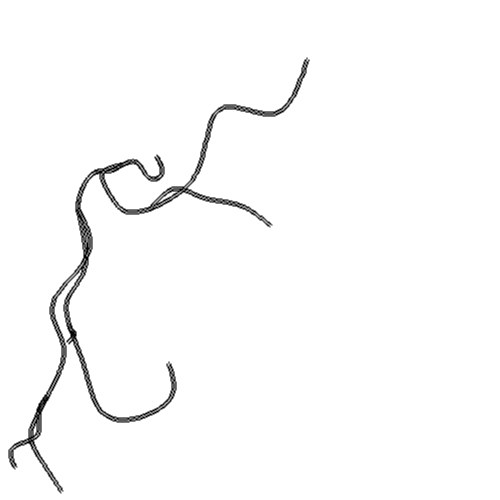
\includegraphics[width=0.4\linewidth]{example_figures/fakeimg.png}
        \caption{An example of the synthetic image of the eleven-segment wire harness}
        \label{An example of the synthetic image of the eleven-segment wire harness}
    \end{figure}
\subsubsection{Operations on segments}
    The dataset could be extended by operations on segments, e.g, rotation and translation. To operate on the branches of the harness, the harness 
    first needs to be segmented. Here the images are firstly segmented to individual segments by using Label-Studio, see \autoref{fig:Wire Segmentation}.\\
	\begin{figure}[!htbp]
		\centering
		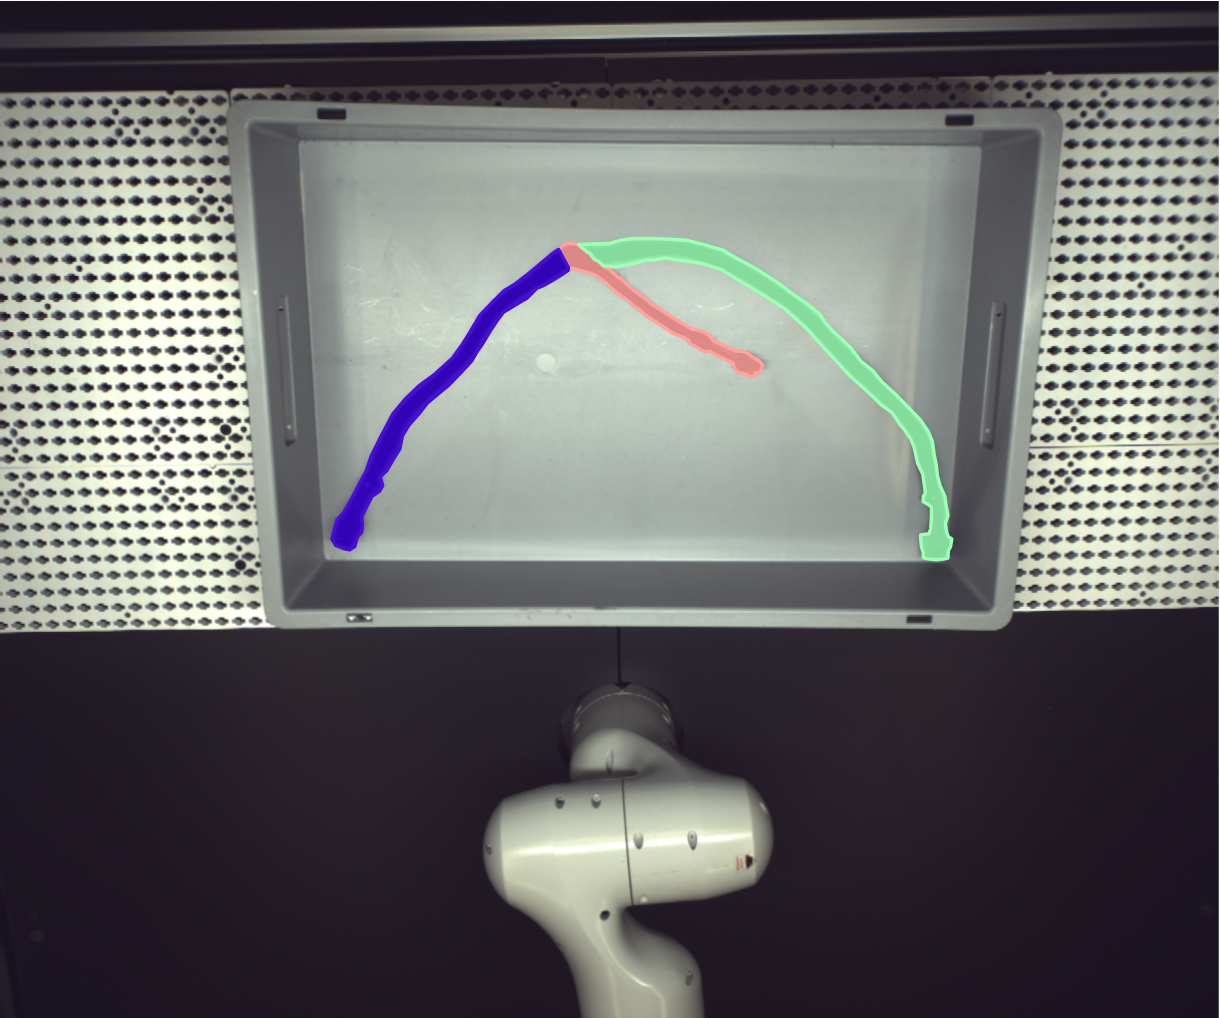
\includegraphics[width=0.6\linewidth]{example_images/img_0_segment}
		\caption{Wire Segmentation}
		\label{fig:Wire Segmentation}
	\end{figure}
	A rotation matrix is defined as \autoref{eq:rotation matrix}:
	\begin{align}
		\begin{bmatrix}
			cos(\theta)&  -sin(\theta )&x \\
			sin(\theta )&  cos(\theta )&y  \\
			0&  0&1
		\end{bmatrix} \label{eq:rotation matrix}
	\end{align}
	An all-zeros mask will be created firstly that has the same size as the image of wire harnesses. The values on mask, where corresponds to the coordinate position of
	annotated points of segmentation, are then equal to one. The corresponding image region $\mho$ of the wire harness will be segmented as a polygonal region based on the mask.
	Build the rotation matrix relative to the desired position and then calculate its corresponding new coordinates by using \autoref{eq:new region}. 
	Paste the previously segmented polygonal area onto the empty background. The new generated virtual image is \autoref{fig:fake image}.
	\begin{align}
		\mho ^{\star } = \mho \cdot \begin{bmatrix}
			cos(\theta)&  -sin(\theta )&x \\
			sin(\theta )&  cos(\theta )&y  \\
			0&  0&1
		\end{bmatrix} \label{eq:new region}
	\end{align}

	\begin{figure}[!htbp]
		\centering
		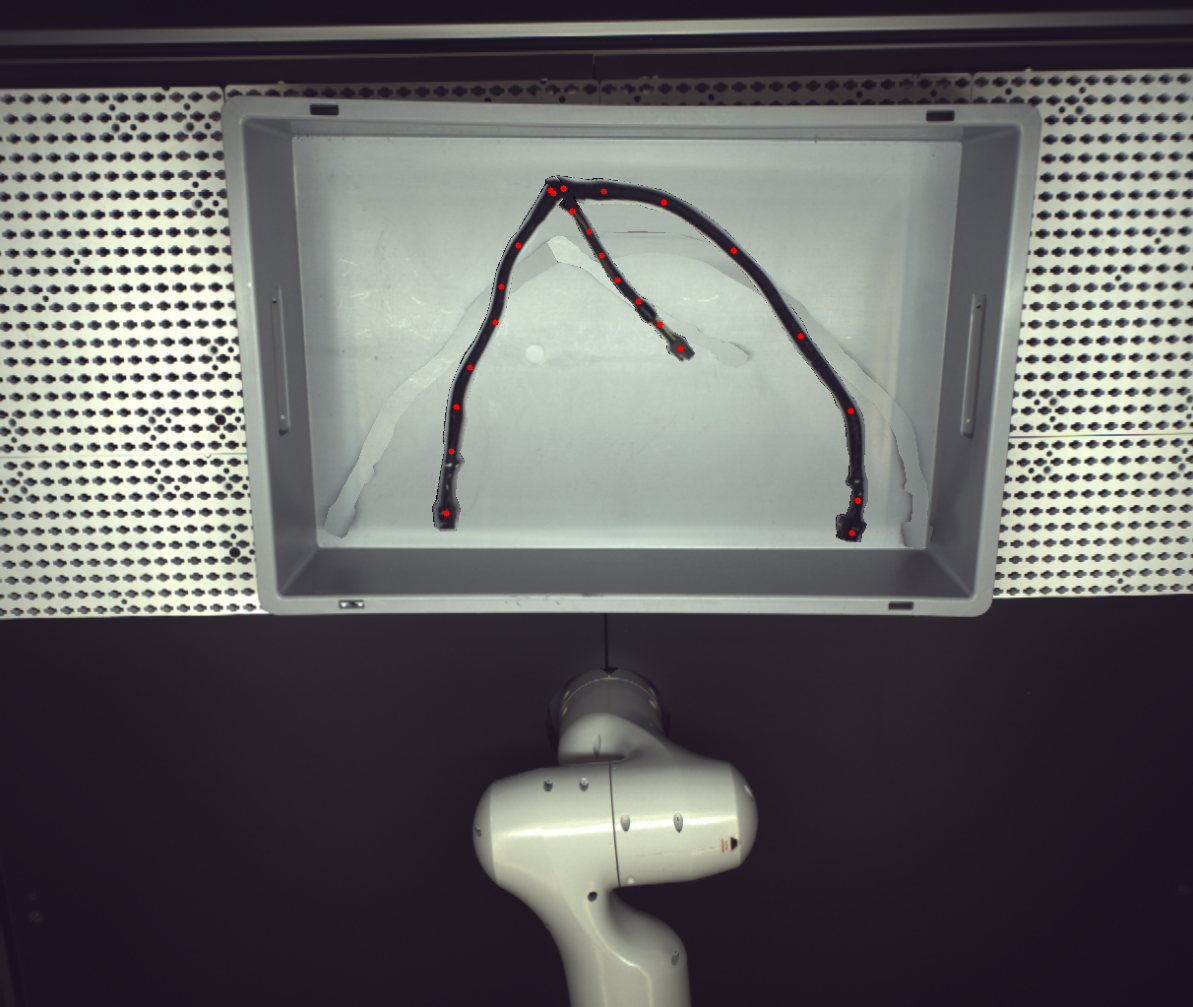
\includegraphics[width=0.6\linewidth]{example_images/img_0_segment_fakeImages}
		\caption{fake image}
		\label{fig:fake image}
	\end{figure}
	The corresponding annotation $\Theta $ could also be calculated with the rotation matrix as \autoref{eq:new anno}:
	\begin{align}
		\Theta ^{\star } = \Theta \cdot \begin{bmatrix}
			cos(\theta)&  -sin(\theta )&x \\
			sin(\theta )&  cos(\theta )&y  \\
			0&  0&1
		\end{bmatrix} \label{eq:new anno}
	\end{align}
\section{Model}
\section{Experiment}